\documentclass[a4paper, 12pt]{article}
\usepackage[margin=24mm]{geometry}
\usepackage{float}
\usepackage{titling}
\usepackage{graphicx}
\usepackage{geometry}
\usepackage{caption}
\usepackage{subcaption}
\usepackage[hidelinks]{hyperref}
\usepackage[toc,page]{appendix}
\usepackage{multirow}
\usepackage{pdfpages}
\usepackage{todonotes}
%
%\geometry{bindingoffset=35mm}
\providecommand{\keywords}[1]{\textbf{\textit{Keywords ---}} #1}

\begin{document}

\listoftodos

\begin{titlepage}
\begin{center}{\LARGE
Electronics and Computer Science\\
Faculty of Physical and Applied Sciences\\
University of Southampton\\
\hfill \break
\hfill \break
\hfill \break\\
Merlin Webster\\
\today\\
\hfill \break
Skydiving Formation Recognition\\
\begin{figure}[H]
	\centering
	\includegraphics[width=.7\linewidth]{fs_silhouette.png}
\end{figure}
Project supervisor: Dr Jonathon S Hare\\
Second examiner: Prof Lie-Liang Yang\\
\hfill \break
\hfill \break
A project report submitted for the award of\\
MEng Electronic Engineering\\}
\end{center}
\end{titlepage}
%

\renewenvironment{abstract}
  {\small\quotation
  {\bfseries\noindent{\large\abstractname}\par\nobreak\smallskip}}
  {\endquotation}
%
\thispagestyle{empty}
\setcounter{page}{0}
\begin{abstract}\textbf{\emph{
	Abstract here...
}}\end{abstract}
\keywords{computer vision, formation skydiving, pose detection, template matching, active shape models}
\clearpage

\textsc{\thispagestyle{empty}
\setcounter{page}{0}
\tableofcontents
\clearpage
\thispagestyle{empty}
\setcounter{page}{0}
\listoffigures 
\clearpage}

\section{Background}
	\subsection{Formation Skydiving}
Skydiving is a competitive and technical sport, requiring careful control of body position in order to move around the sky in a controlled manner whilst in free-fall.\\
A popular discipline in the sport is formation skydiving (FS). This involves multiple skydivers forming set shapes with their bodies, in order to score as many points as possible.
		\subsubsection{Rules}
		A point is awarded for each successful formation in a sequence \textbf{\emph{(see figure \ref{fig:fs_dive_pool})}}. A successful formation is defined only by the correct hands of each skydiver holding the correct grips on the other skydivers \textbf{\emph{(see figure \ref{fig:grips})}}, and not by the orientation of the skydivers themselves.
%
\begin{figure}[H]
	\centering
	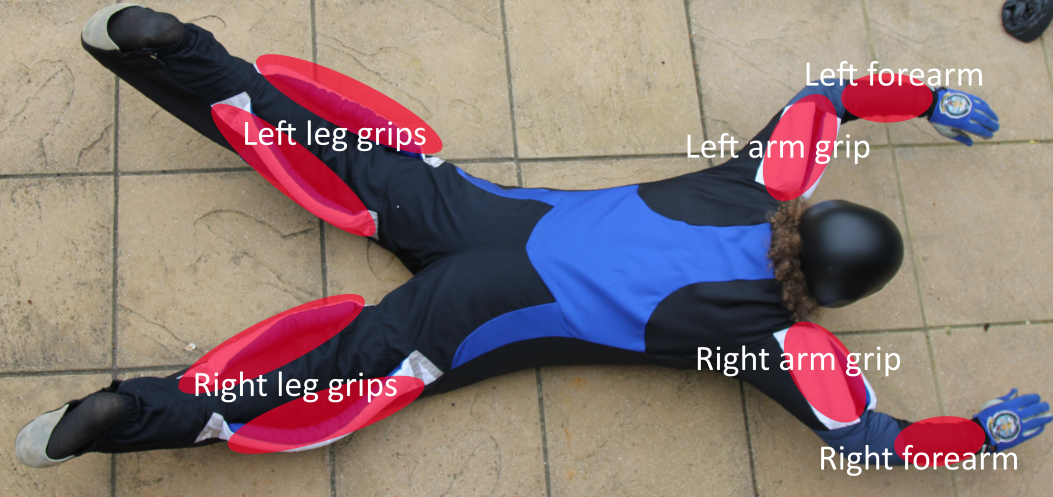
\includegraphics[width=0.9\linewidth]{grips.png}
	\caption{Diagram showing all of the available grips on a formation skydiving suit.}
	\label{fig:grips}
\end{figure}
%
\noindent In 4 person FS (4-way FS) each skydiver has a specific slot in the formation. This is the position that they will always take when making each formation. This is done in such a way that the amount of movement required for each skydiver when transitioning between formations is minimised. The four slots in 4-way FS are known as Point, Tail, Outside Center (OC) and Inside Center (IC). 
%
	\subsubsection{Training Practices}
In order for the team to create formations in the sky, it is important that they practice the skydive multiple times on the ground. This is known as "dirt diving" and is often done using partially triangular wheeled platforms that each skydiver lays on, known as "creepers"  \textbf{\emph{(see figures \ref{fig:creepers} and \ref{fig:creepers_use})}}.
\begin{figure}[H]
	\centering
	\begin{subfigure}{.5\textwidth}
		\centering
		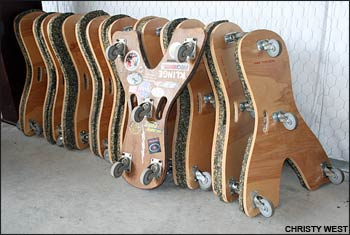
\includegraphics[width=0.9\linewidth]{creepers.jpg}
		\caption{FS practice platforms "creepers"}
		\label{fig:creepers}
	\end{subfigure}%
	\begin{subfigure}{.5\textwidth}
		\centering
		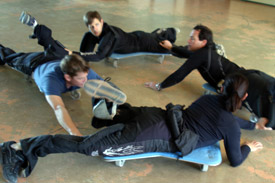
\includegraphics[width=0.9\linewidth]{creepers_use.jpg}
		\caption{"Creepers" in use while "dirt diving" a "Donut" formation}
		\label{fig:creepers_use}
	\end{subfigure}
	\caption{Images reproduced from \url{www.skydivespaceland.com/blog/images/creepers2.jpg} and \url{www.skydiveaz.com/images/old-images/creepers.jpg}}
\end{figure}
%
\noindent Another way that FS teams train is to use a vertical (indoor skydiving) wind tunnel. A fan is mounted at the bottom or bottom of the tunnel creating a strong wind that the skydivers can float on; simulating the environment of a regular skydive, but in a much more controlled environment \textbf{\emph{(see figure \ref{fig:sample_tunnel})}}.
	\subsection{Project Brief}
The original focus of the project was to analyse video of dirt diving and identify which formations have been performed. The focus has been changed slightly, and is now to analyse footage of formation skydiving in a vertical wind tunnel. This change is largely due to the fact that the body position of a skydiver free-fall is much more similar to their body position in a wind tunnel, than when dirt diving. Another benefit of analysing footage taken in a wind tunnel is that the camera is mounted above the formation, remaining static \textbf{\emph{(see figure \ref{fig:sample_tunnel})}}. This allows the skydivers to much more easily be separated from the background via background subtraction\cite{Piccardi}. The set of formations that will be analysed are the BPA rookie class of formations known as 'randoms'. The software must be able to recognise all 16 of the randoms \textbf{\emph{(see figure \ref{fig:fs_dive_pool})}}.
%
\begin{figure}[H]
	\centering
	\includegraphics[width=\linewidth]{FS_All.png}
	\caption{All 16 BPA rookie class FS 'randoms' formations, with their names. The colours for each slot are: Point red, OC green, IC blue, Tail yellow.\\
	Reproduced from \url{http://www.teamsatori.co.uk/New\%204W\%20Random\%20Dive\%20pool.pdf}}
	\label{fig:fs_dive_pool}
\end{figure}
%
\begin{figure}[H]
	\centering
	\begin{subfigure}{.5\textwidth}
		\centering
		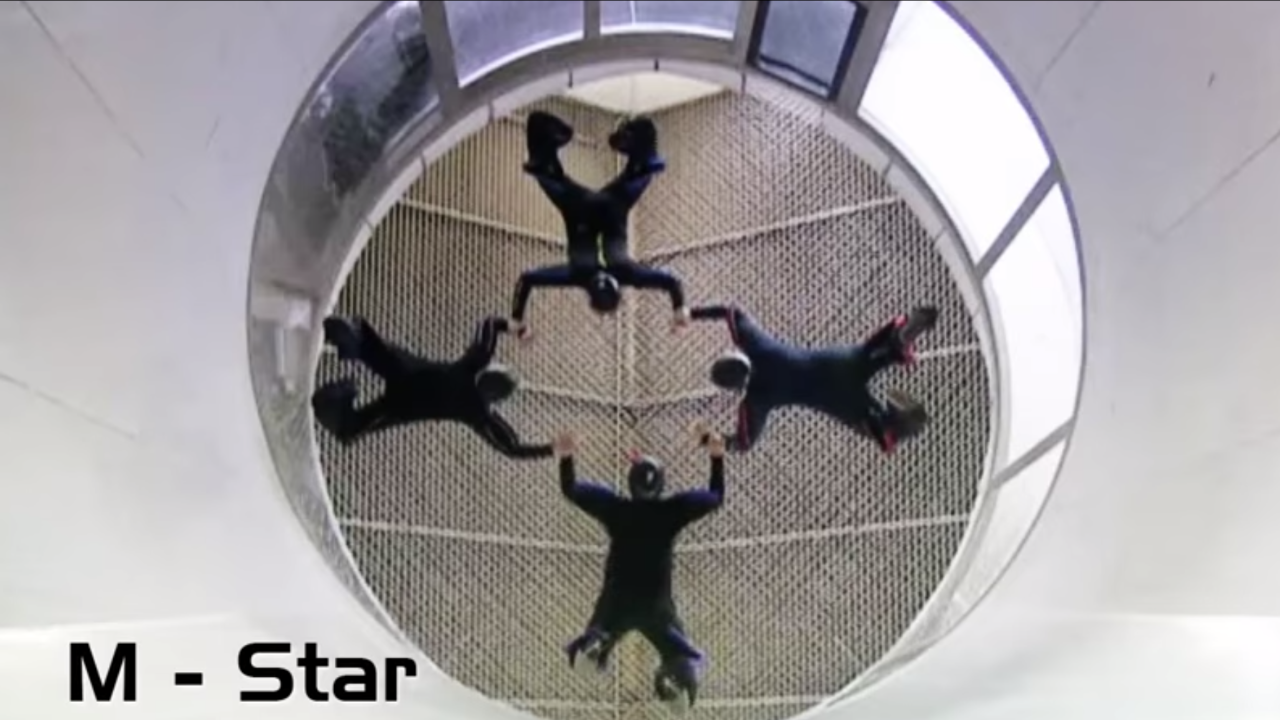
\includegraphics[width=0.9\linewidth]{Tunnel_Star.png}
	\end{subfigure}%
	\begin{subfigure}{.5\textwidth}
		\centering
		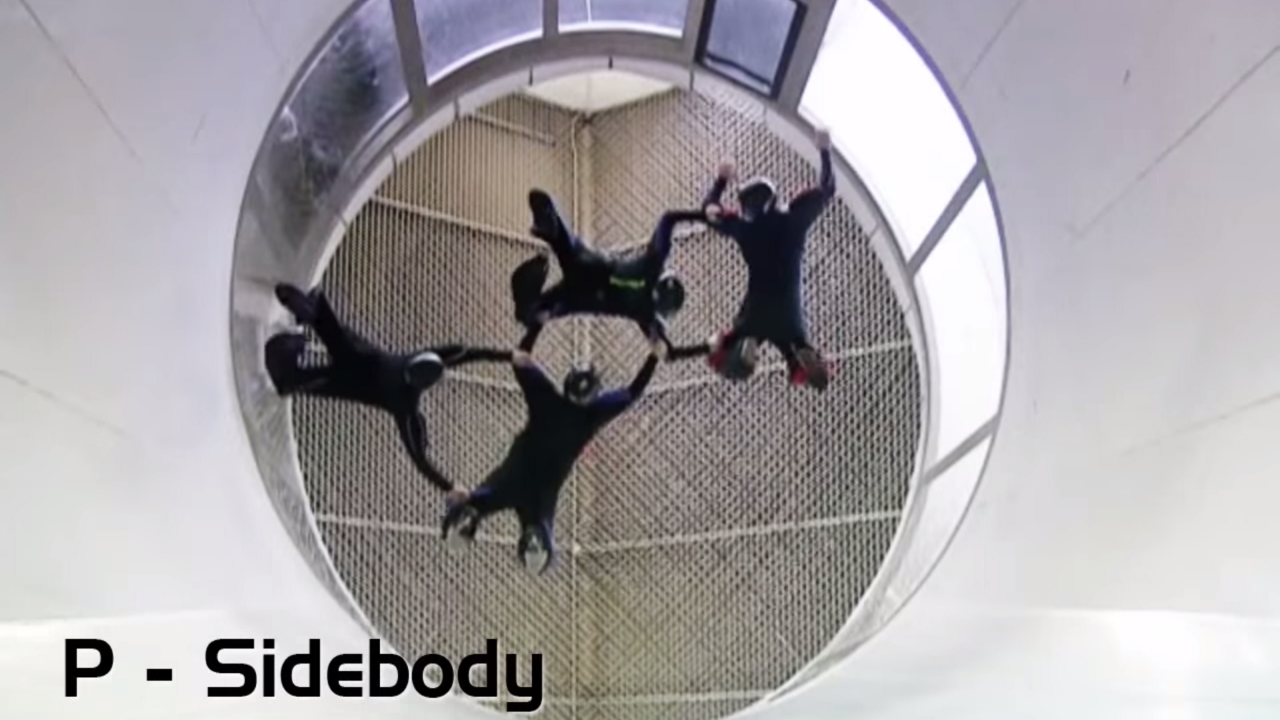
\includegraphics[width=0.9\linewidth]{Tunnel_Sidebody.png}
	\end{subfigure}\\
	\begin{subfigure}{.5\textwidth}
		\centering
		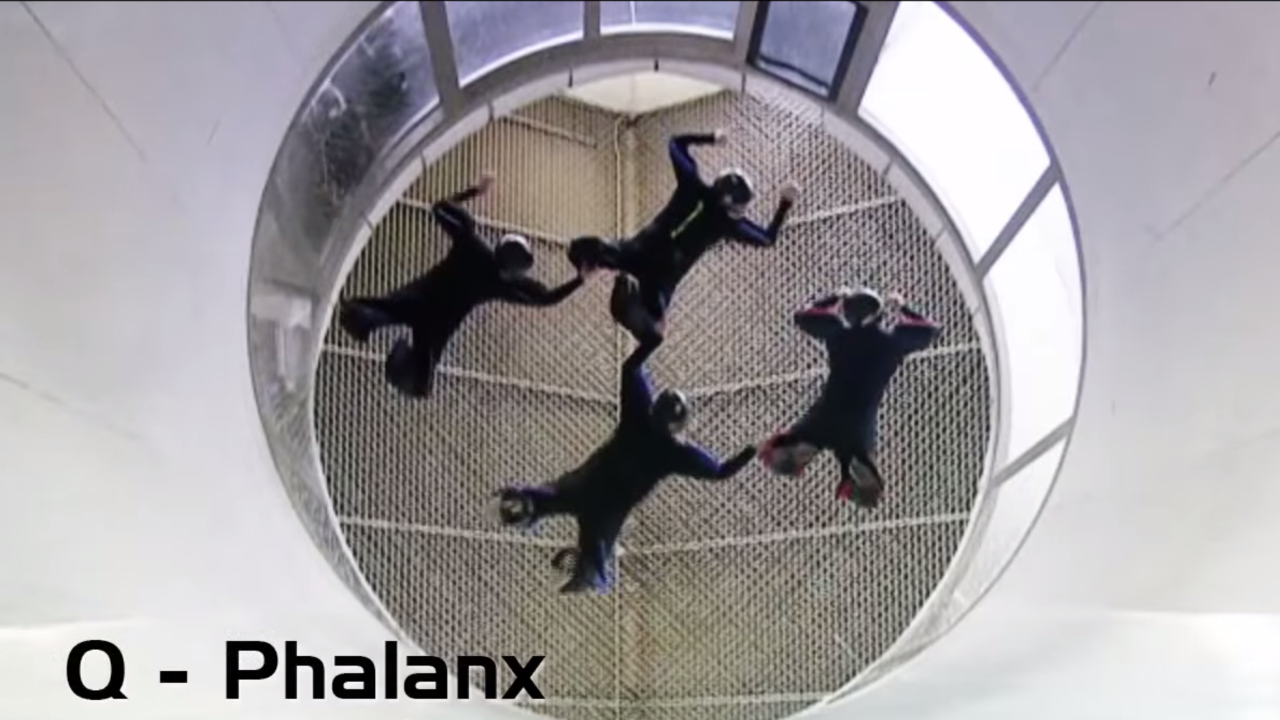
\includegraphics[width=0.9\linewidth]{Tunnel_Phalanx.png}
	\end{subfigure}%
	\begin{subfigure}{.5\textwidth}
		\centering
		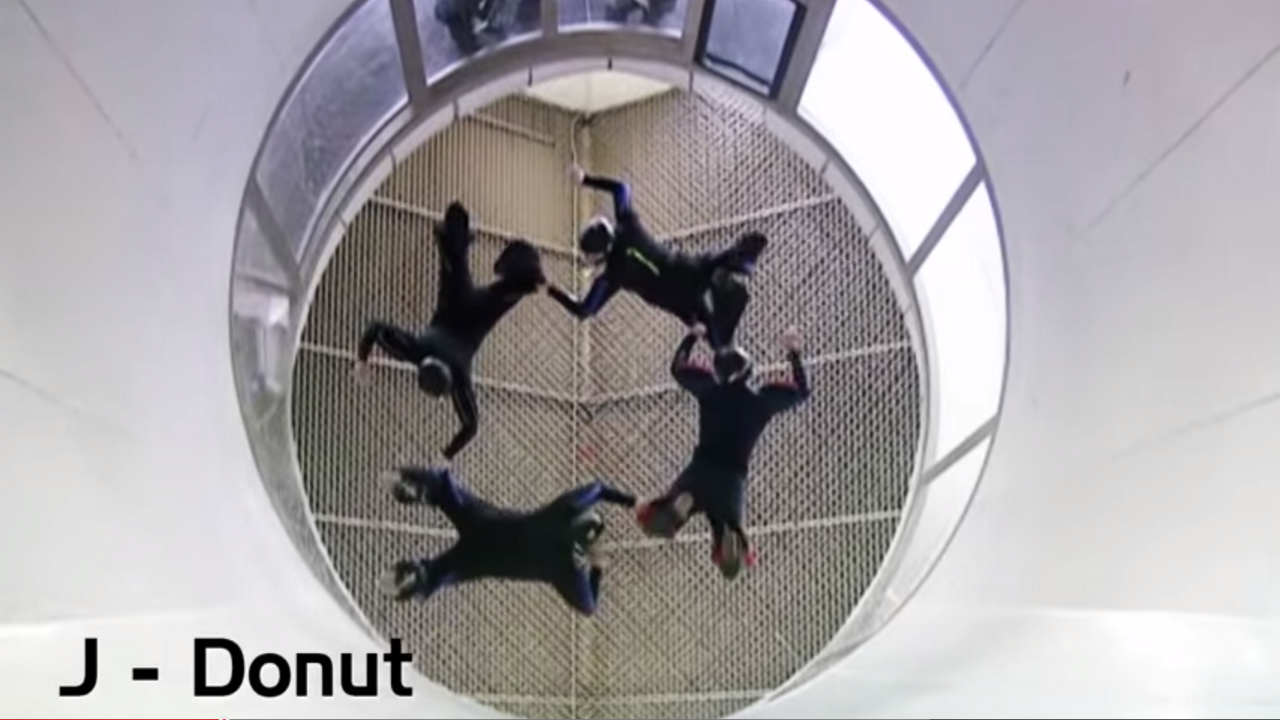
\includegraphics[width=0.9\linewidth]{Tunnel_Donut.png}
	\end{subfigure}%
	\caption{Sample FS formations performed in a wind tunnel, with their names.\\
	Images reproduced from International Bodyflight Association, \url{www.youtube.com/watch?v=Y2B4S3lGf54&list=LLsEkKn0qzIHSGefmSGT_4og}. }
	\label{fig:sample_tunnel}
\end{figure}
%
\noindent An image of a skydiver in an FS body position can be simplified to a set of line segments between 11 key points; one for the waist, neck, head, left and right hands, elbows, knees and feet \textbf{\emph{(see figure \ref{fig:stick_model_fitted})}}.
%
\begin{figure}[H]
	\centering
	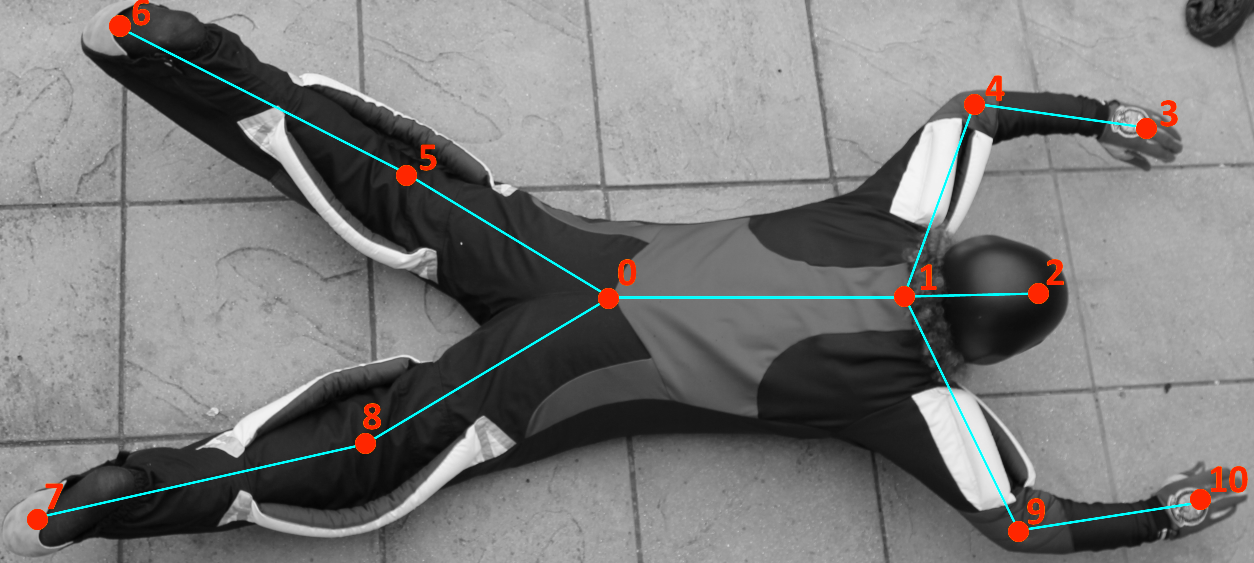
\includegraphics[width=\linewidth]{stick_model_fitted.png}
	\caption{Diagram showing how an image of a skydiver can be simplified to a set of line segments between 11 points.}
	\label{fig:stick_model_fitted}
\end{figure}
%
\section{Literature Report}
%
Due to the specialist nature of the project, relevant existing literature is somewhat limited.
However, there does exist relevant literature on various methods for human posture recognition.

\subsection{Pose Detection}
%
Human pose detection can be a difficult problem to tackle; many factors contribute towards this, such as shadows, occlusions, complicated backgrounds and noisy source images.\\
There are many different proposed methods to tackle the task of human posture detection; over a wide variety of technologies. Some methods use depth cues extracted from 3d scanner information, such as \cite{kinect_IR} which uses a Microsoft Kinect to detect the human body. Other methods are designed to work with video\cite{video}, creating a 3d estimation of human pose in order to detect people. A common goal is to try to detect the pose of a person from a single static image. There are a variety of ways of doing this such as, using a model-based method, where an explicit pose model must be specified, often requiring complicated 3d modelling and rendering\cite{model-based}. Another method used relies on texture cues in order to perform "Parts-based" object detection\cite{monocular_still_images}, this method neither uses an explicit model, or pre-labelled data.\\
However, the method that is deemed to most fit goal of recognising the pose of a skydiver is an adaptive method, such as Active Shape Models. Active Shape Models are more often used in facial feature detection\cite{cootes}\cite{face_recognition}; given that it only relies on a set of simple points, labelled from a set of training images it should be ideal for the task at hand.
%
\subsection{Active Shape Models}
Active Shape Models are statistical shape models that are able iteratively deform in order to fit a given example image. They can also be used to characterise the ways in which a set of points in an image can move. Using principal component analysis\cite{icl_pca}, it is possible to find a minimal set of feature variables which control the overall shape of an object. Varying these enables every possible permutation of the set of image points to be found.\\
In order for this to be done, a training set of points must be collected by hand from images similar to those that will be analysed. This This training set of points forms the initial point matrix.
%
\begin{figure}[H]
	\centering
	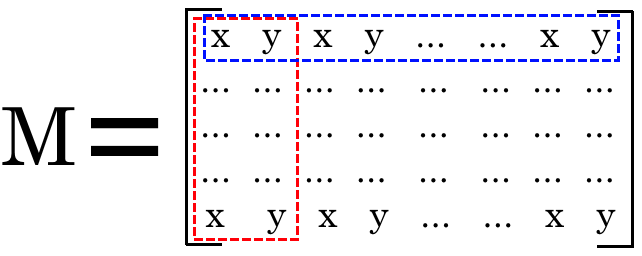
\includegraphics[width=.5\linewidth]{shape_matrix.png}
	\caption{Initial point matrix. Each row corresponds to a different image (blue). Pairs of columns contain coordinates of the same point across each of the images (red).}
	\label{fig:shape_matrix}
\end{figure}
%
\noindent The iterative algorithm generalised procrustes analysis (GPA) is then used to optimally rotate, scale, and translate the points from each image. The goal of this is to have the points from each image match as closely as possible when superimposed on each other \textbf{\emph{(see figure \ref{fig:procrastes})}}.
%
\begin{figure}[H]
	\centering
	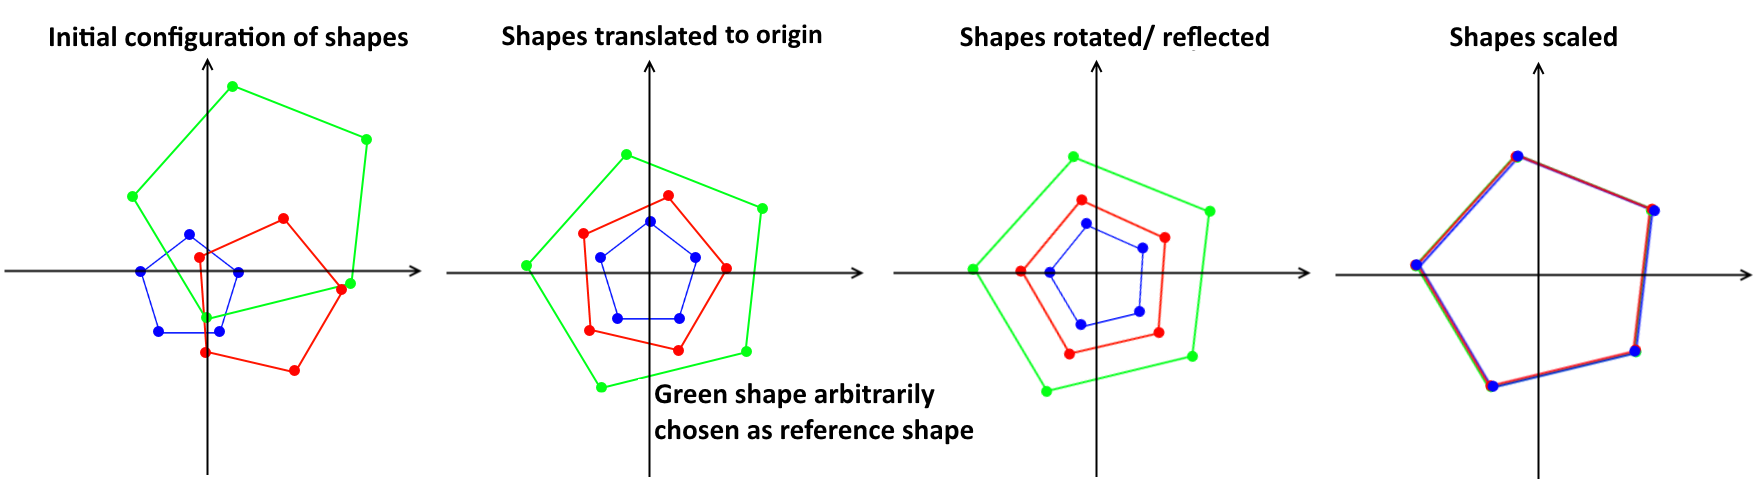
\includegraphics[width=\linewidth]{generalised_procrastes_ananlysis.png}
	\caption{Performing generalised procrustes analysis on three shapes.}
	\label{fig:procrastes}
\end{figure}
%
\noindent A shape matrix can be created using the same format as the initial point matrix, but containing the coordinates of the aligned image points.
Finally, principal component analysis is used to reduce the dimensions of the shape matrix. This is done by finding the eigenvalues and eigenvectors of the covariance matrix. A more in depth explanation can be found at \cite{icl_pca}.\\
\\
Using this method it is possible to find weather a skeleton of a skydiver is viable or not. This is done by creating the initial point matrix from a set of images of a skydiver in a variety of FS body positions. The resulting active shape model will contain information defining how a skydiver's body position can change. A set of test points that make up the skydiver's skeleton \textbf{\emph{(see figure \ref{fig:stick_model_fitted})}} can then be compared to this model to find if the skeleton is possible or not. This allows the skeleton to be recalculated, should it be found to be impossible.
%
%
\subsection{Template Matching}


\section{Problem Analysis and Specification}
\todo[inline]{Define terms to be used somewhere, e.g. landmark model, skydiver mask}
\section{Final System Design}
%	Run down of main program flow. Reference appendix for flowchart

	\subsection{Computing Background Image}
	%median image of video
	\subsection{Foreground Extraction}
		\subsubsection{Binary Median Filter}
	The classic way of doing a median filter is to apply a median go through each point in the image, and take the surrounding
	8 pixels values, sort them by value, pick the median, and use that as the new value for the central pixel.
	However, for a binary image, this process can be optimised.
	Since we know each pixel will either be 0 or 1, it is unnecessary to sort the values of the surrounding pixels
	,instead they are just added, and the total examined. If the total is greater than 4, then
	the median is 1, and 0 otherwise.\\
	This can be efficiently implemented by creating an n by n mask filled 
	with ones, and convolving it with the binary image to create a new greyscale image with each pixel containing the sum of
	it's neighbours. The image is then thresholded at 4.5, causing any pixel which had more neighbours containing ones than zeroes
	to take the value of 1, and any with more 0 neighbours to take the value of 0
	This gives the same result as applying the median filter in the classic way, but with much lower computation time, as only convolution and thresholding 	are required.
	\todo[inline]{Add a figure for each step, with comparison images of classic way, and binary optimisation}
	\todo[inline]{Add a figure to show the ones mask used}
	%
	\subsection{Rotation Metric}
		\subsubsection{Image Moments}
		\todo[inline]{Mention principle components, and how the formula conveniently  resembles that of image moments, and give formulae for calculation image moments. Second image moment.}
		Another method that was tried was to find the minimum area rotated rectangle of the mask, and take it's angle to be the major axis of the 				skydiver. 
		OpenCV has a function for finding the minimum area rectangle. Unfortunately, the angle it returns is the perpendicular angle to the rectangle's
		side closest to 0 degrees. This means that if this angle were used for the major axis, it may be 90, 180, or 270 degrees off.
		As a result, this method could not be used.
		\todo[inline]{Add a figure showing the min area rotated rect around the skydiver mask, with the major axis drawn, and the the
		angle returned from the min area rotated rect drawn.}
		\subsubsection{Skydiver Orientation}
		The major axis defines the angle of the line that runs along the skydivers spine.
		The line will either point towards the skydivers head, or crotch, but it is not possible to know which.
		This meant that the angle returned from the function to calculate the major axis was often off by 180 degrees.\\
		In order to test if the angle calculated points towards the head or feet of the skydiver,
		the assumption is made that the distance from the skydivers centroid to their groin will be less
		than the distance from their centroid to their head.
		These distances are calculated by starting at the centroid, and then iteratively moving a
		test point further away in the direction of the major axis angle
		This is done until the test point is no longer in the skydiver mask.
		This gives the first distance, labelled the 'up' distance.
		The second distance, the 'down' distance, is found by repeating the process, but instead moving the
		test point in the direction 180 degrees from the major axis angle.
		The distances are then compared, and if the 'down' distance is greater than the 'up' distance
		the major axis angle is thought to be 180 degrees out.
		In this case 180 degrees is added or subtracted
		accordingly, so as to make sure the angle stays in the range 0 - 360 degrees.
		\todo[inline]{Add figures showing the up and down distances labelled on the skydiver mask}
%
	\subsection{Translation Metric}
	%1.Image moments, first moment
	%2. Centroid of points
	%Center point of the minimum area rotated rectangle could also be used for this
	Another method that could be used is to find the minimum area rotated rectangle enclosing the skydiver mask or landmark model.
	The center point of the rotated rectangle would then be assumed to be the center point of the mask or landmark model.
	However, this would only work if the mask or landmark model was symmetric. 
	If this was not the case, this method would give an incorrect centroid point.
	\todo[inline]{include figure showing skydiver mask centroid using the two methods, demonstrating that the min area rect center does not work.)}
	
	\subsection{Scale Metric}
	%Centroid size formula
	A scale metric was required in order to compare the sizes of different binary images, and contours.
	\todo[inline]{Add an explanation as to why this was required at the top of the section.}
	Two separate methods were tried in order to find a reliable metric that could be used to compare the sizes of different binary images, and contours.
	The first of which was to use the centroid size, which is the square root of the summed squared distances from each point to the centroid.
	\todo[inline]{Include centroid size equation and ref}
	While this could be used to compare the relative size of the landmark model between iterations, it was not useful when comparing the size of the binary
	mask to the landmark model.\\
	\todo{define how "it was not useful"}
	The method that was finally employed was to find the minimum area rotated rectangle enclosing the landmark model, or binary mask, and use it's enclosed 	area as a scale metric. This proved to be more reliable when comparing the landmark model to a binary mask.
	\subsection{Template Matching}
	%Move a template accross the image and calculate how much it fits at each point
	%Take find the area of greatest fit from the resulting image 
	\subsection{Model Plausibility Test}
	%Project model points using the PCA model
	%Check the resulting components are with n std deviations of the mean
	%the std deviation varies for each component, and is lower for each subsequent component
	%talk about PCA demo tool & reference that part of the report
	%constrain the components by clipping them down to +- n std deviations if they are outside this range
	%(Box constraint)
	%Project the points back to get get new model
	%PCA removes all scale, rotation, and translation information from the model
	%Scale, rotate, and translate the model, using information from procrustes analysis
	\subsection{Model Initialisation}
	\subsubsection{Finding Skydivers}
	\todo[inline]{Add a figure for each step}
	The purpose of this part of the system was to find a suitable frame to be used in order to create the initial contours, and binary masks of the 			skydivers.
	This frame should clearly show four separate skydivers, who are not touching.
	This was achieved in the following way:
	\begin{enumerate}
		\item Take a greyscale frame from the source video 
		\item Perform background subtraction on the frame in order to get an approximate binary mask of the skydivers
		\item Apply the binary median filter to
		\item Find the external contours of the binary mask
		\item Calculate the standard deviation of the area of the list of contours
		\item Keep only contours whose area is greater than one standard deviation of the mean area
		\item Sort the remaining contours by area, in descending order
		\item Take the four largest contours to represent the four skydivers.
	If less than four four contours remain after removing the smaller contours, then go back to step 1.
	\end{enumerate}
	If four contours with an area greater than one standard deviation of the mean cannot be found, it is likely to be for one of the following reasons:
	\begin{itemize}
		\item The frame was not an image of the four skydivers as expected
		\item The frame was an image of the four skydivers, but two or more of the skydivers were touching.
		This would be the case if a formation was made. This failure would occur because the external contour of the overlapping skydivers would be seen as 		a single contour, and thus the number of contours of an appropriate size would be less than four.
		\item The calculated background image was not representative of the video background
	\end{itemize}
	%
	Only finding the external contours caused any internal contour information to be lost.
	This meant that when the contours were drawn to create the binary masks, any gaps between the skydivers were filled unintentionally.
	This was fixed by creating a second mask image that retained the hole information, and taking the final
	skydiver blobs as the result of performing the logical AND operation on the two masks.
	\todo[inline]{Add a figure to demonstrate this as well}
%
	\subsection{Formation Detection}
	
	\subsection{Landmark Collection Tool}
	In order to create the landmark model, a training set of landmarks must first be collected.
	These landmarks could then be used to perform principle component analysis \todo[inline]{Ref} and collect the templates \todo[inline]{Ref}.
	A separate program was written to do this whose function is as follows:
	\begin{enumerate}
		\item Load a training video of skydivers performing 4-way formation skydiving in the wind tunnel
		\item Take a number of sample frames from this video
		\item On each frame the user clicks on each landmark position in the order waist, neck, head, left hand, left elbow, left knee, left foot,
		right foot, right knee, right elbow, right hand, as shown in figure \textbf{\emph{(see figure \ref{fig:stick_model_fitted})}}
		\item The user then presses space in order to save the collected points
		\item A stick man is then drawn over the points that were just labelled in order to verify that they were collected correctly
		\item This is done four times, once for every skydiver in the frame, allowing 4 sets of landmarks to be collected for every frame
		\item This process is repeated for each sample frame, and the data is saved to a file in the matrix format shown in \textbf{\emph{figure \ref{fig:shape_matrix}}}
	\end{enumerate}
	Each frame used to collect landmarks is also saved as an image to be used by the template creation program.
	
	
	%Idea is to display a frame from the source video, and then mark the 11 key points on each of the 4
	%skydivers in the frame
	%Left click to add a point, right click to remove one, middle click to skip frame
	%Space bar to save the 11 key points labelled
	%Once all the skydivers are labelled the another frame is displayed and the process continues
	%Once all the points are collected, they are saved in a matrix
	%Rows contain 22 values, 11 sets of points x0,y0,x1,y1,....x10,y10 The 11 points form a keypoint vector
	%Each new row stores another keypoint vector
	%Every frame used to collect landmarks is saved so that it can be used to create templates
	%Talk about how a binary image mask of the skydiver blobs is also stored for each frame
	%Include screenshots of consol window, alongside frame with skeletons drawn on it
	
	\subsection{Template Creation Tool}
	In order to perform template matching, a template image for each landmark must be made.
	A separate program was written to do this.
	As it's input it takes the landmark matrix, and saved frames produced by the landmark collection program.
	It then takes rotation independent samples of each frame, centred at each of the landmarks, and creates
	a template image for each landmark point.
	The template images are calculated as mean of all of the samples for that landmark point.
	Taking the mode of the samples was also considered as a possibility, but this method 
	%The idea is to create a general template for each part of the skydiver: hands, elbows, head etc.
	%These templates would later be used to perform templpate matching on the frames in order to refine
	%the keypoints in the skydiver model
	%Talk about subimg extraction function:
	%Use two points to define the rotation for each sample, the point being sampled, and some reference
	%List each central point, and it's reference point
	%Talk about how the angle is calculated from these two points (just trig)
	%Create a rotated rect at the center point, at the angle calculated, with a width and height
	%Equal to how large the templates should be
	%Collect A subimg for every point in the input matrix, 11 per keypoints vector
	%Take the mean of all of the subimages for each keypoint to get a template for that key point
	%Talk about how a binary mask subimage is also taken for each point
	%It was originally done becasue the mean of the subimages always tended to be black,
	%and it was assumed that this was becuase taking the mean of the background was causing
	%the image to cancel out and equal zero. The binary mask was used to prevent this by removing
	%the background before taking the mean of the subimages.
	%It was later found that the black templates were due to the method the mean was being taken
	%All of the subimages would be summed, then divided by the number of subimages
	%As each image was stored with 8-bits, a maximum value of 256, the sum of the images would quickly
	%reach the maximum value, and clip at 256.
	%This meant that when the sum images were divided by the number of subimages used, they would always appear
	%to be black.
	%This was fixed by taking the mean in a different way, taking the cumulative mean
	%Include both mean formulas
	%Using the cumulative mean prevented the template being created from ever becoming too bright
	%This allowed a mean image of each keypoint subimage to be calculated.
	%These mean templates were then saved
	\subsection{Principle Component Analysis Tool}
		\subsubsection{Generalised Procrustes Analysis}
		
		\subsubsection{Principle Component Analysis}

%
%
\section{System Implementation}
\noindent In order to complete this project C++ will be used, making use of the open source computer vision library OpenCV 3.0\cite{\cite{OpenCV}} in order to reduce the time required to perform standard tasks, such as loading an image file, or receiving a video feed.
%

\section{Additional Work}

	\subsection{Principle Component Analysis Demonstration}

	\subsection{Skeletonisation}
	Software has been written that creates a minimal, connected, 1 pixel thick skeleton from a binary mask. The function uses a medial axis transformation based method \cite{skeletonisation}  to create the skeleton and the Ramer--–Douglas–--Peucker\cite{Ramer}\cite{Douglas_Peucker} (RDP) algorithm to minimise it.
%
	\subsubsection{Skeletonisation Algorithm}
        \begin{enumerate}
   		\item Find all boundary pixels (edge of the binary mask) using a binary laplacian mask\cite{binary_laplacian}. For each boundary pixel do the following:
        \item{Test pixels neighbours
        %
\begin{table}[H]
\centering
\begin{tabular}{llll}
\cline{1-3}
\multicolumn{1}{|l|}{p8} & \multicolumn{1}{l|}{p1} & \multicolumn{1}{l|}{p2} & y \\ \cline{1-3}
\multicolumn{1}{|l|}{p7} & \multicolumn{1}{l|}{p0} & \multicolumn{1}{l|}{p3} &  \\ \cline{1-3}
\multicolumn{1}{|l|}{p6} & \multicolumn{1}{l|}{p5} & \multicolumn{1}{l|}{p4} & $\downarrow$ \\ \cline{1-3}
x &  & $\rightarrow$ & 
\end{tabular}
\end{table}}
%
        \item Count Np0, number of non-zero neighbours of p0.
        \item Count Tp0, number of 0-1 transitions in sequence p1, p2, ..., p8.
        \item Check the initial conditions; mark for deletion any point that satisfies them all.\\
        Initial conditions:
        \begin{itemize}
         \item $cA:     2 <= Np0 <= 6$
         \item $cB:     Tp1 = 1$
         \item $cC:     p1 . p3 . p5 = 0$
         \item $cD:     p3 . p5 . p7 = 0$
         \end{itemize} 
         
        \item Delete any points marked for deletion.
        \item For each remaining boundary pixel, recalculate Np0 and Tp0, then check secondary conditions; marking for deletion any point that satisfies them all:\\
Secondary conditions:
        \begin{itemize}
        \item $cA:     2 <= Np0 <= 6$
        \item $cB:     Tp1 = 1$
        \item $cC\_:    p1 . p3 . p7 = 0$
        \item $cD\_:    p1 . p5 . p7 = 0$
        \end{itemize}
        \item Delete any points marked for deletion.
        \end{enumerate}
%
Repeat process until no points are deleted.\\
For more a more in depth explanation of the algorithm, see \cite{skeletonisation}.\\
\\
Initially a simpler algorithm\cite{skeletonisation_simple} was used in order to create the skeleton using morphological operations to perform thinning. However, this algorithm did not ensure that the skeleton created was minimal or connected, and was therefore insufficient.
\begin{figure}[H]
	\centering
	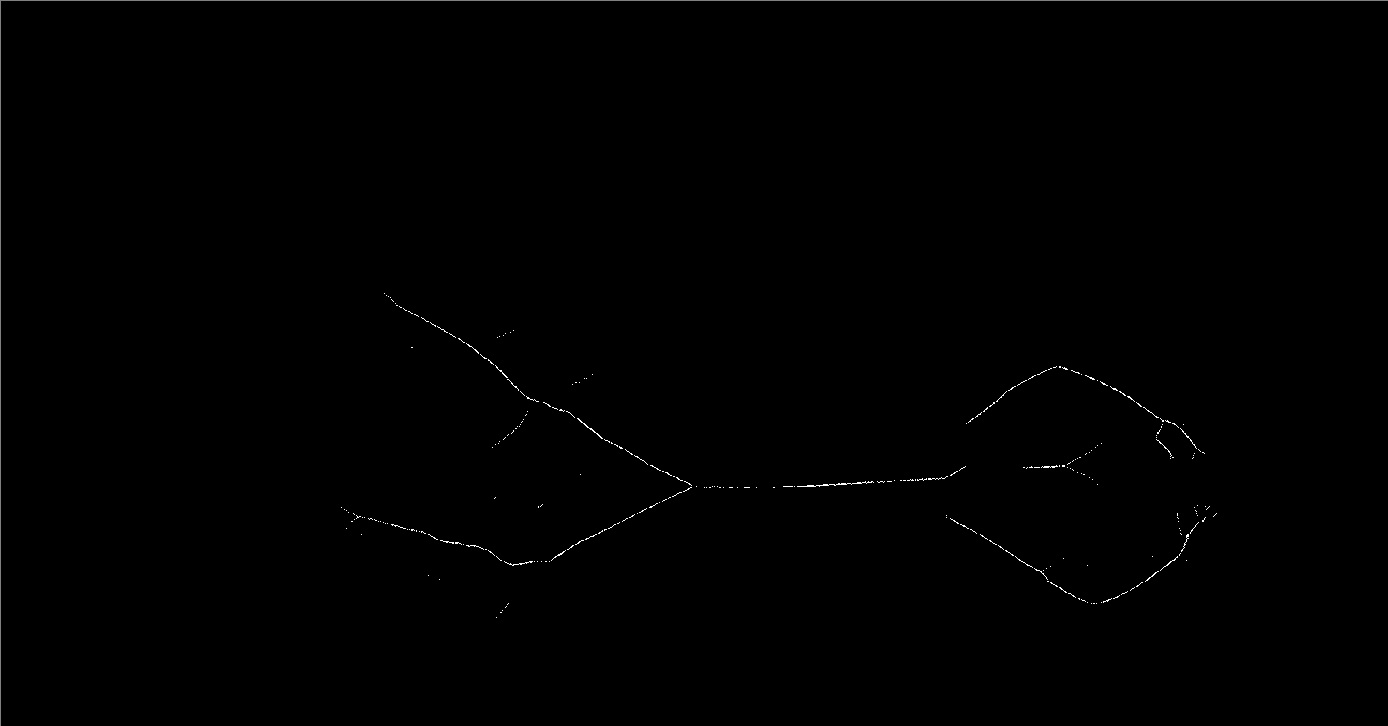
\includegraphics[width=\linewidth]{skel_simple.jpg}
	\caption{Result of using the morphological thinning algorithm on the binary image shown in \textbf{\emph{figure \ref{fig:skel_src_mask}}}.}
	\label{fig:skel_simple}
\end{figure}
		\subsubsection{Skeleton Simplification Algorithm}
	The RDP algorithm is designed to simplify a curve, while still maintaining its overall shape. A curve can be thought of as a collection of linked line segments, with each line segment stretching between two consecutive points on the curve. The basic principle of the algorithm is to reduce the number of line segments in a curve; creating a similar, but simplified curve. The algorithm is initially given an ordered array of all the points in the curve. The algorithm is also given the variable $\epsilon$; this defines the degree to which the curve should be simplified and represents a minimum distance between line segments on the curve. It marks the start and end points of the curve as the first line segment (L), and then finds the point furthest from this initial line segment. If the distance from this point to the line segment (d) is less than $\epsilon$ then it is marked for removal. If the point is further than $\epsilon$ then it is kept and the algorithm recursively called with this point as the new end point. In this way the algorithm is able to remove every point that is closer than $\epsilon$ to the line segment that joins its neighbours.
%
\begin{figure}[H]
	\centering
  	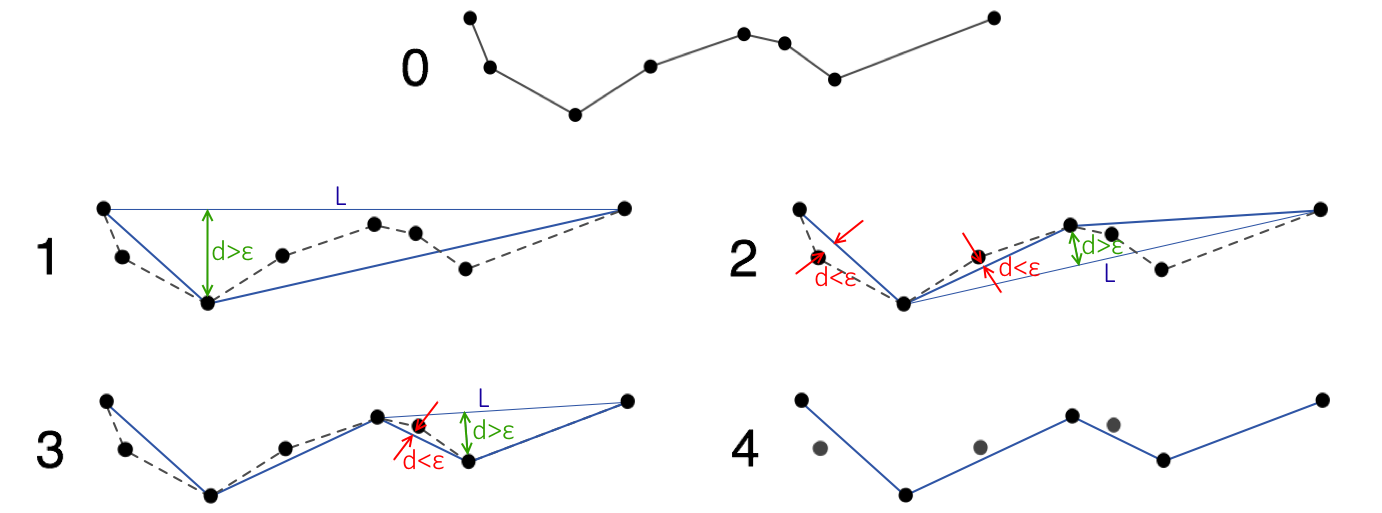
\includegraphics[width=\textwidth]{douglas_peucker.png}
  	\caption{Diagram showing the RDP algorithm working on a curve. 0 being the initial curve to be simplified, and 4 being the fourth result the algorithm. Red arrows show points marked for deletion, green arrows show points to be kept\\
  	Modified from \url{http://upload.wikimedia.org/wikipedia/commons/9/91/Douglas_Peucker.png}.}
  	\label{fig:douglas_peucker}
\end{figure}
%
\noindent The RDP algorithm is used to reduce the number of points in the skeleton, simplifying it; however, it is only able to simplify curves with no bifurcations. This proves to be a problem when trying to simplify a skeleton produced by the skeltonisation algorithm, as it will always have bifurcations at the waist and neck. It may also also produce erroneous bifurcations at other points on the skeleton. These bifurcations can be seen in \textbf{\emph{figure \ref{fig:skel}}}.\\
The location of these bifurcations can be detected by applying a modified version of condition $cB$ from the skeletonisation algorithm. Tp0 is calculated in the same way, by looking at the number of 0-1 transitions in the sequence p1, p2, ... , p8.
%
\begin{table}[h]
\centering
\begin{tabular}{llll}
\cline{1-3}
\multicolumn{1}{|l|}{p8} & \multicolumn{1}{l|}{p1} & \multicolumn{1}{l|}{p2} & y \\ \cline{1-3}
\multicolumn{1}{|l|}{p7} & \multicolumn{1}{l|}{p0} & \multicolumn{1}{l|}{p3} &  \\ \cline{1-3}
\multicolumn{1}{|l|}{p6} & \multicolumn{1}{l|}{p5} & \multicolumn{1}{l|}{p4} & $\downarrow$ \\ \cline{1-3}
x &  & $\rightarrow$ & 
\end{tabular}
\end{table}
%
\\If $Tp0 > 2$ then a bifurcation is present at p0.
This is always true, as the skeletonisation algorithm ensures that the skeleton is a single pixel thick 8-connected component.\\
Once the location                               of every bifurcation is found, the skeleton can be split into separate curves, by removing the bifurcation point. The RDP algorithm is then run on each of these curves independently. The simplified curves can then be recombined to form a simplified skeleton. At this point it is also possible the remove the false skeleton sections created by the skeletonisation algorithm forming erroneous bifurcations. The simplest way to do this is to delete any simplified skeleton section that is shorter than a given length. This works as the false skeleton sections tend to be shorter than the correct ones. A more reliable method for detecting false skeleton sections could be used in the final design.
\begin{figure}[H]
	\centering
	\begin{subfigure}{.5\textwidth}
  		\centering
  		\includegraphics[width=.95\linewidth]{skel_src.jpg}
  		\caption{Skeletonisation source image.}
  		\label{fig:skel_src}
	\end{subfigure}%
	%
	\begin{subfigure}{.5\textwidth}
  		\centering
  		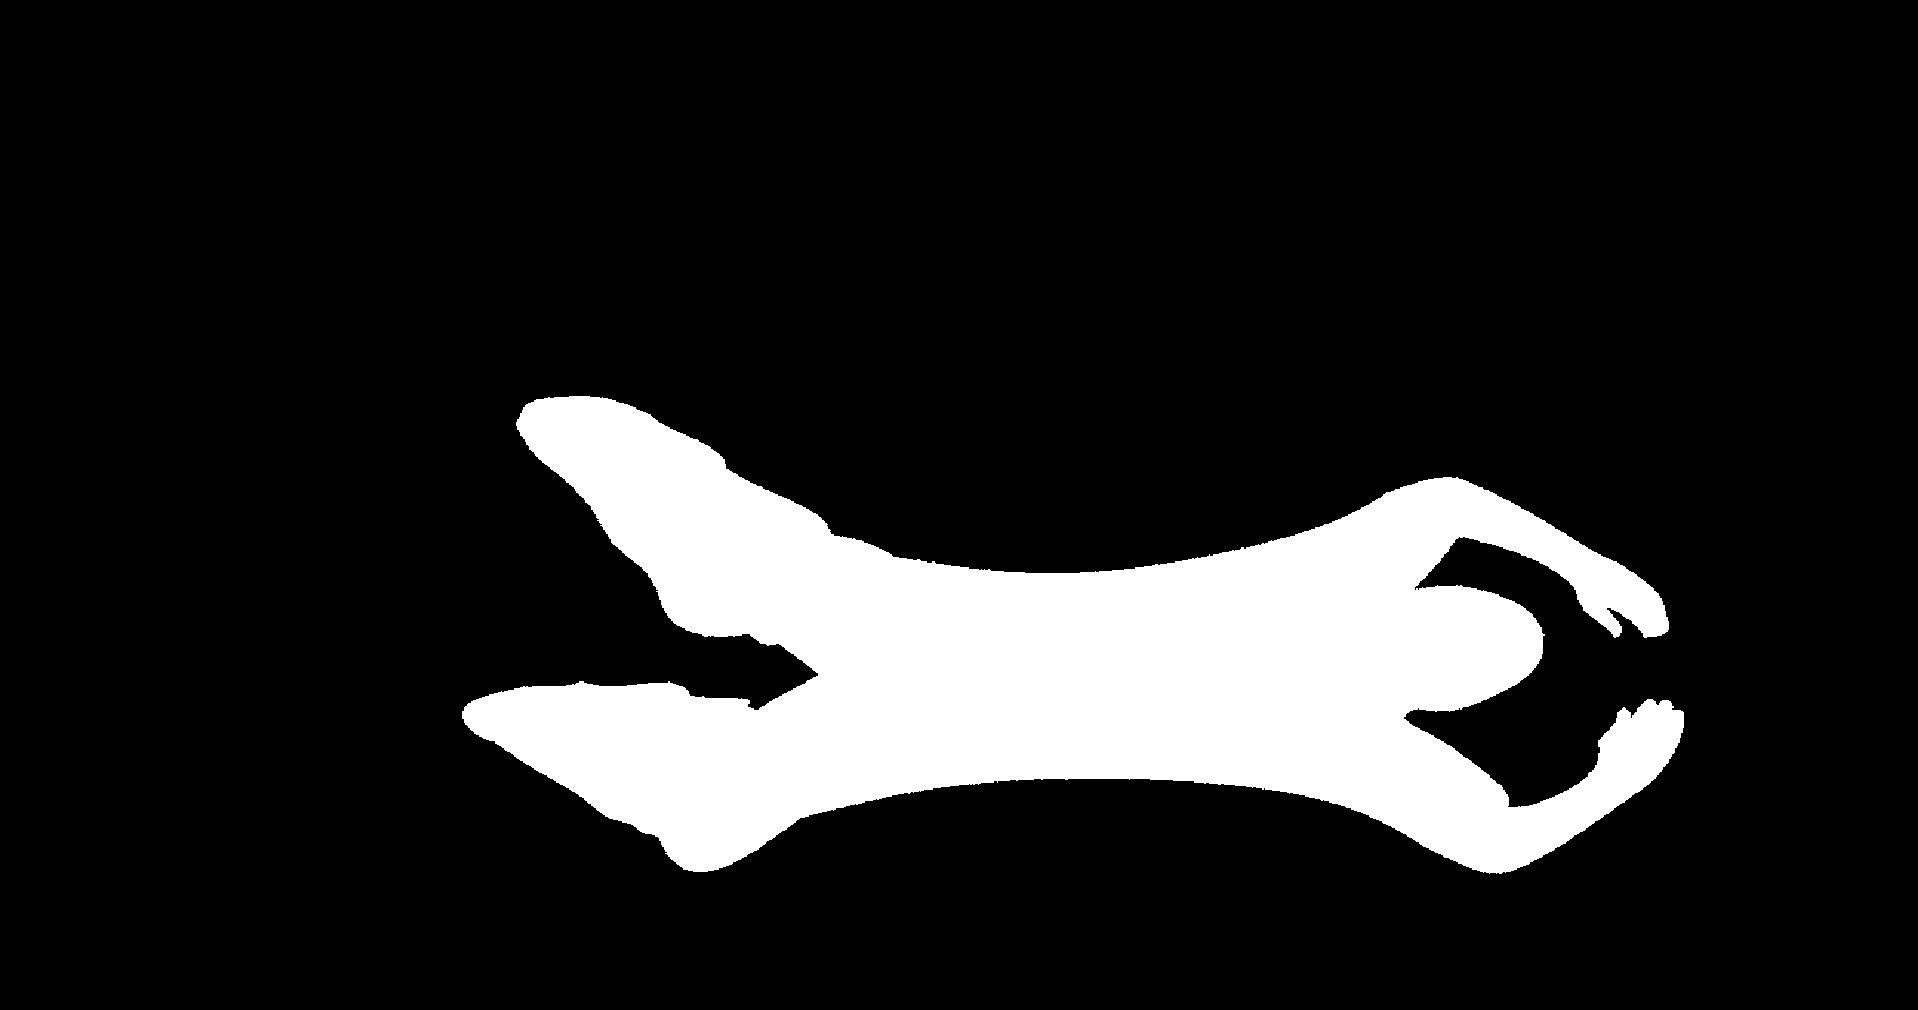
\includegraphics[width=.95\linewidth]{skel_src_mask.jpg}
  		\caption{Binary mask of source image.}
  		\label{fig:skel_src_mask}
	\end{subfigure}\\
	%
	\begin{subfigure}{\textwidth}
  		\centering
  		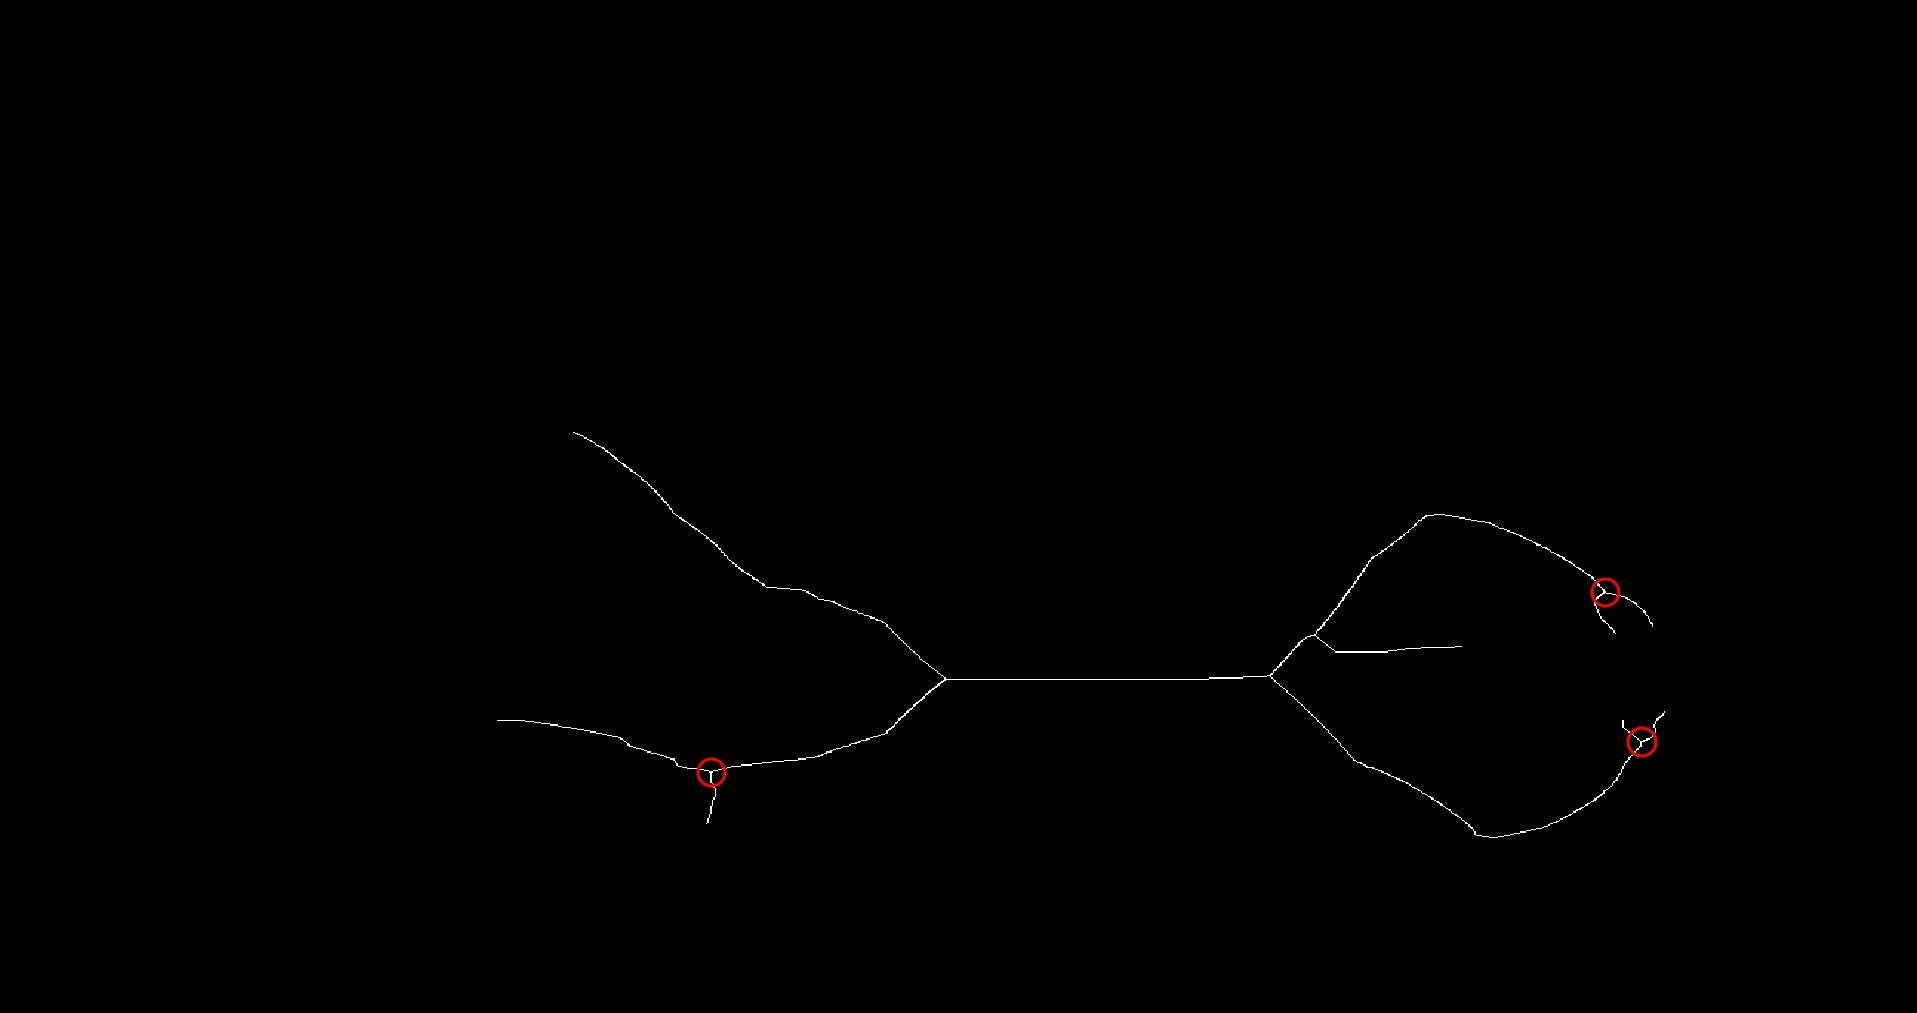
\includegraphics[width=\linewidth]{skel.jpg}
  		\caption{Result of skeletonisation function. Erroneous bifurcations are circled in red.}
  		\label{fig:skel}
	\end{subfigure}\\
	%
	\begin{subfigure}{\textwidth}
  		\centering
  		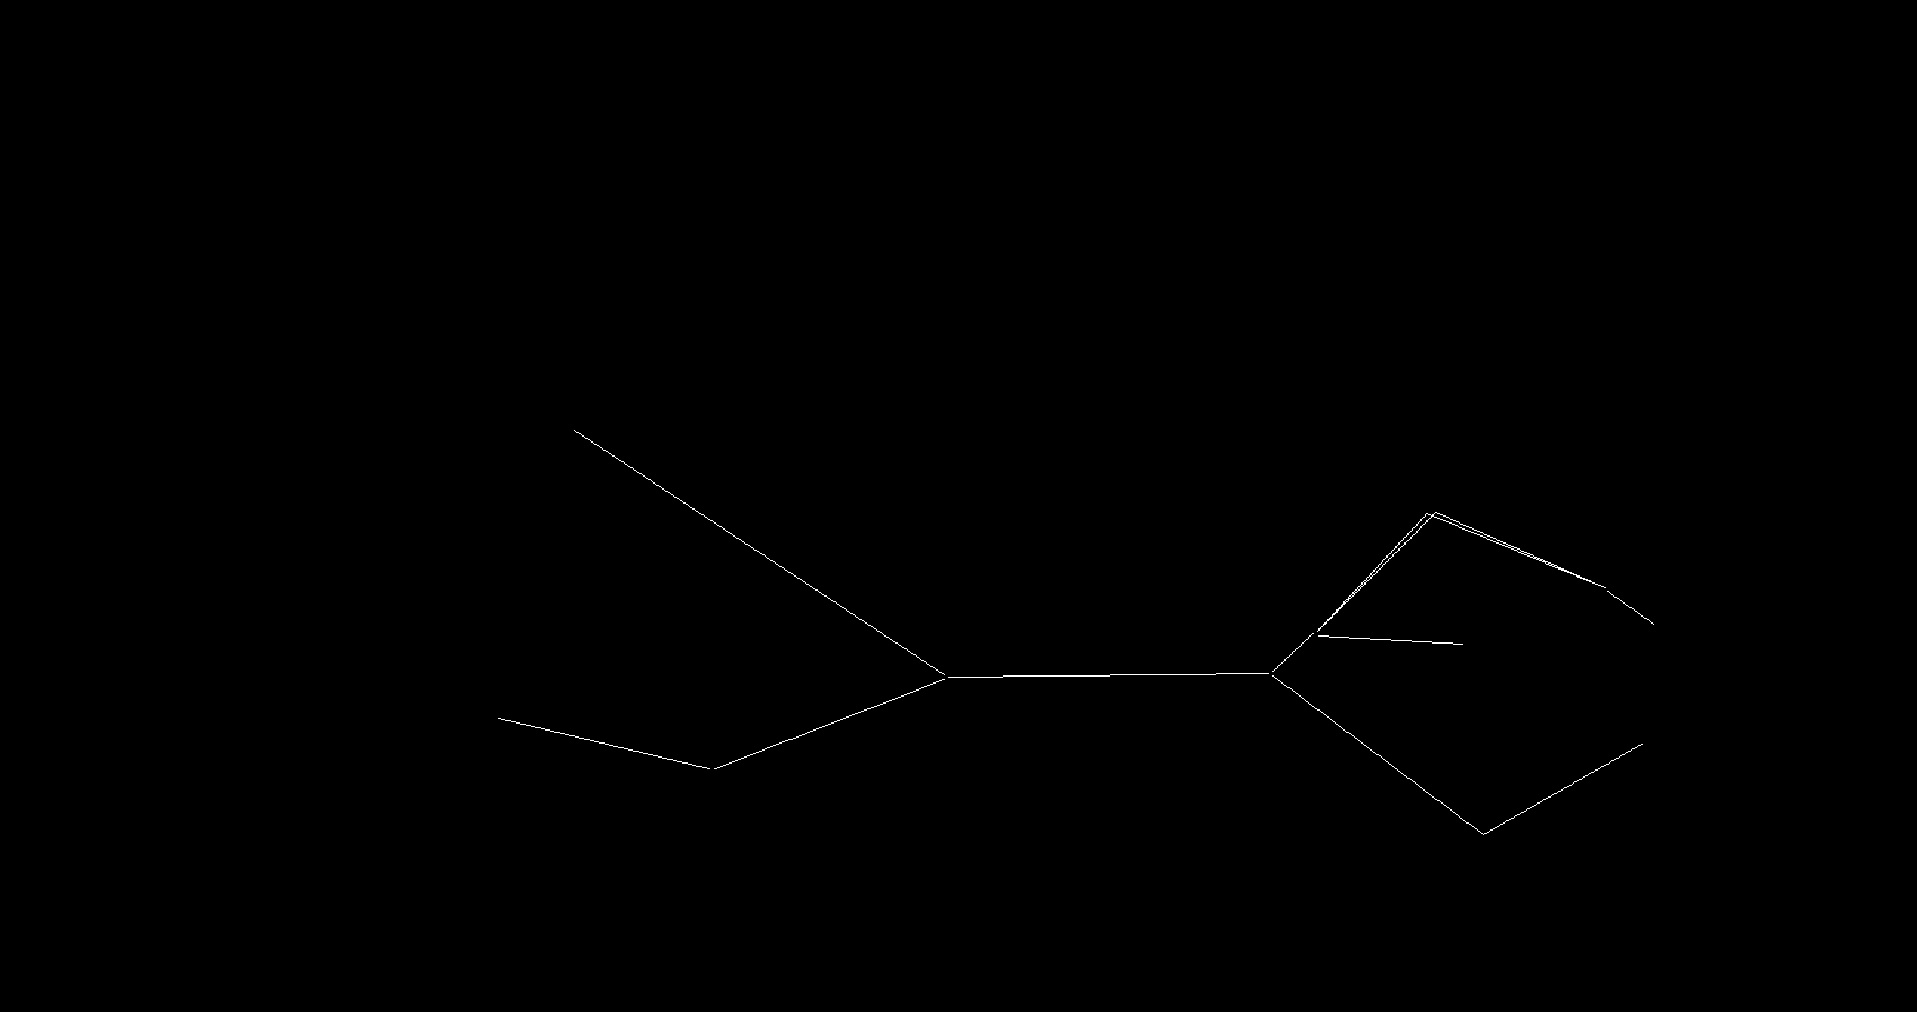
\includegraphics[width=\linewidth]{skel_reduced.jpg}
  		\caption{Result of skeleton simplification algorithm.}
  		\label{fig:skel_reduced}
	\end{subfigure}
\caption{Results of skeletonisation and simplification algorithms.}
\end{figure}
%

\section{Project Management}

\section{Conclusion}
	\subsection{Critical Evaluation}
	\subsection{Future Work}

%
%
\clearpage
\begin{thebibliography}{9}
\bibitem{skeletonisation}
    Rafael C. Gonzalez \& Richard E. Woods,
    "Skeletons",
    Digital Image Processing -- Second Edition --- International Edition (2001),
    pg650-653
%
\bibitem{skeletonisation_simple}
    Rafael C. Gonzalez \& Richard E. Woods,
    "Skeletons",
    Digital Image Processing -- Second Edition --- International Edition (2001),
    pg543-545
%
\bibitem{binary_laplacian}
    Rafael C. Gonzalez \& Richard E. Woods,
    "The Laplacian",
    Digital Image Processing -- Second Edition --- International Edition (2001),
    pg581-585
%
\bibitem{Ramer}
    Urs Ramer,
    "An iterative procedure for the polygonal approximation of plane curves",
    Computer Graphics and Image Processing (1972),
    pg 244--–256
%
\bibitem{Douglas_Peucker}
	David Douglas \& Thomas Peucker,
	"Algorithms for the reduction of the number of points required to represent a 				digitized line or its caricature",
	The Canadian Cartographer (1973),
	pg112--–122
%
\bibitem{icl_pca}
	Imperial College London,
	"Lecture 15: Principal Component Analysis",
	\url{www.doc.ic.ac.uk/~dfg/ProbabilisticInference/IDAPILecture15.pdf},
	Last access: 9 Dec 2014
%
\bibitem{cootes}
	Tim Cootes, E. R. Baldock, \& J. Graham,
 	"An introduction to active shape models.",
 	Image Processing and Analysis(2000),
 	pg223---248
%
\bibitem{Piccardi}
	Piccardi, M., "Background subtraction techniques: a review," Systems,
	Man and Cybernetics,
	2004 IEEE International Conference,
	pg3099---3104 vol.4, 		
	(10-13 Oct 2004),
	doi: 10.1109/ICSMC.2004.1400815
%
\bibitem{OpenCV}
	OpenCV,
	"The OpenCV Reference Manual
	Release 2.4.9.0"(April 21, 2014),
	\url{http://docs.opencv.org/opencv2refman.pdf},
	Last access: 09 Dec 2014
%
\bibitem{Qt}
	Qt Project,
	"Qt Reference Pages",
	QtDoc 5.3,
	\url{http://docs.opencv.org/opencv2refman.pdf},
	Last access: 09 Dec 2014
%
\bibitem{2d_pose_detection}
	"Automatic Detection of 2D Human Postures Based
on Single Images",
	QtDoc 5.3,
	\url{http://docs.opencv.org/opencv2refman.pdf},
	Last access: 09 Dec 2014
%
\bibitem{monocular_still_images}
	Wachs, Juan P., Deborah Goshorn, and Mathias Kolsch,
	"Recognizing human postures and poses in monocular still images."(2009),
%
\bibitem{kinect_IR}
	Lu Xia, Chia-Chih Chen, Aggarwal, J.K.,
	"Human detection using depth information by Kinect,"
	Computer Vision and Pattern Recognition Workshops (CVPRW),
	2011 IEEE Computer Society Conference on , vol.,
	no., pp.15,22, 20-25 June 2011
doi: 10.1109/CVPRW.2011.5981811
%
\bibitem{video}
	Yu Tsz-Ho, Tae-Kyun Kim, and Roberto Cipolla,
	"Unconstrained monocular 3d human pose estimation by action detection and cross-			modality regression forest.",
	In Computer Vision and Pattern Recognition (CVPR),
	2013 IEEE Conference on, pp. 3642-3649. IEEE, 2013.
%
\bibitem{model-based}
Christophe Doignon (2007),
An Introduction to Model-Based Pose Estimation and 3-D Tracking Techniques,
Scene Reconstruction Pose Estimation and Tracking, Rustam Stolkin (Ed.), ISBN: 978-3-902613-06-6, InTech, pg360-376,
Available from:
\url{http://www.intechopen.com/books/scene_reconstruction_pose_estimation_and_tracking/an_introduction_to_m
odel-based_pose_estimation_and_3-d_tracking_techniques}
%
\bibitem{face_recognition}
Prabhu, Utsav, and Keshav Seshadri,
"Facial Recognition Using Active Shape Models, Local Patches and Support Vector Machines."
%
\end{thebibliography}
\clearpage
\begin{appendices}
%
\chapter{\textbf{A - Final System Flowchart}}
\label{appendix:system_flowchart}
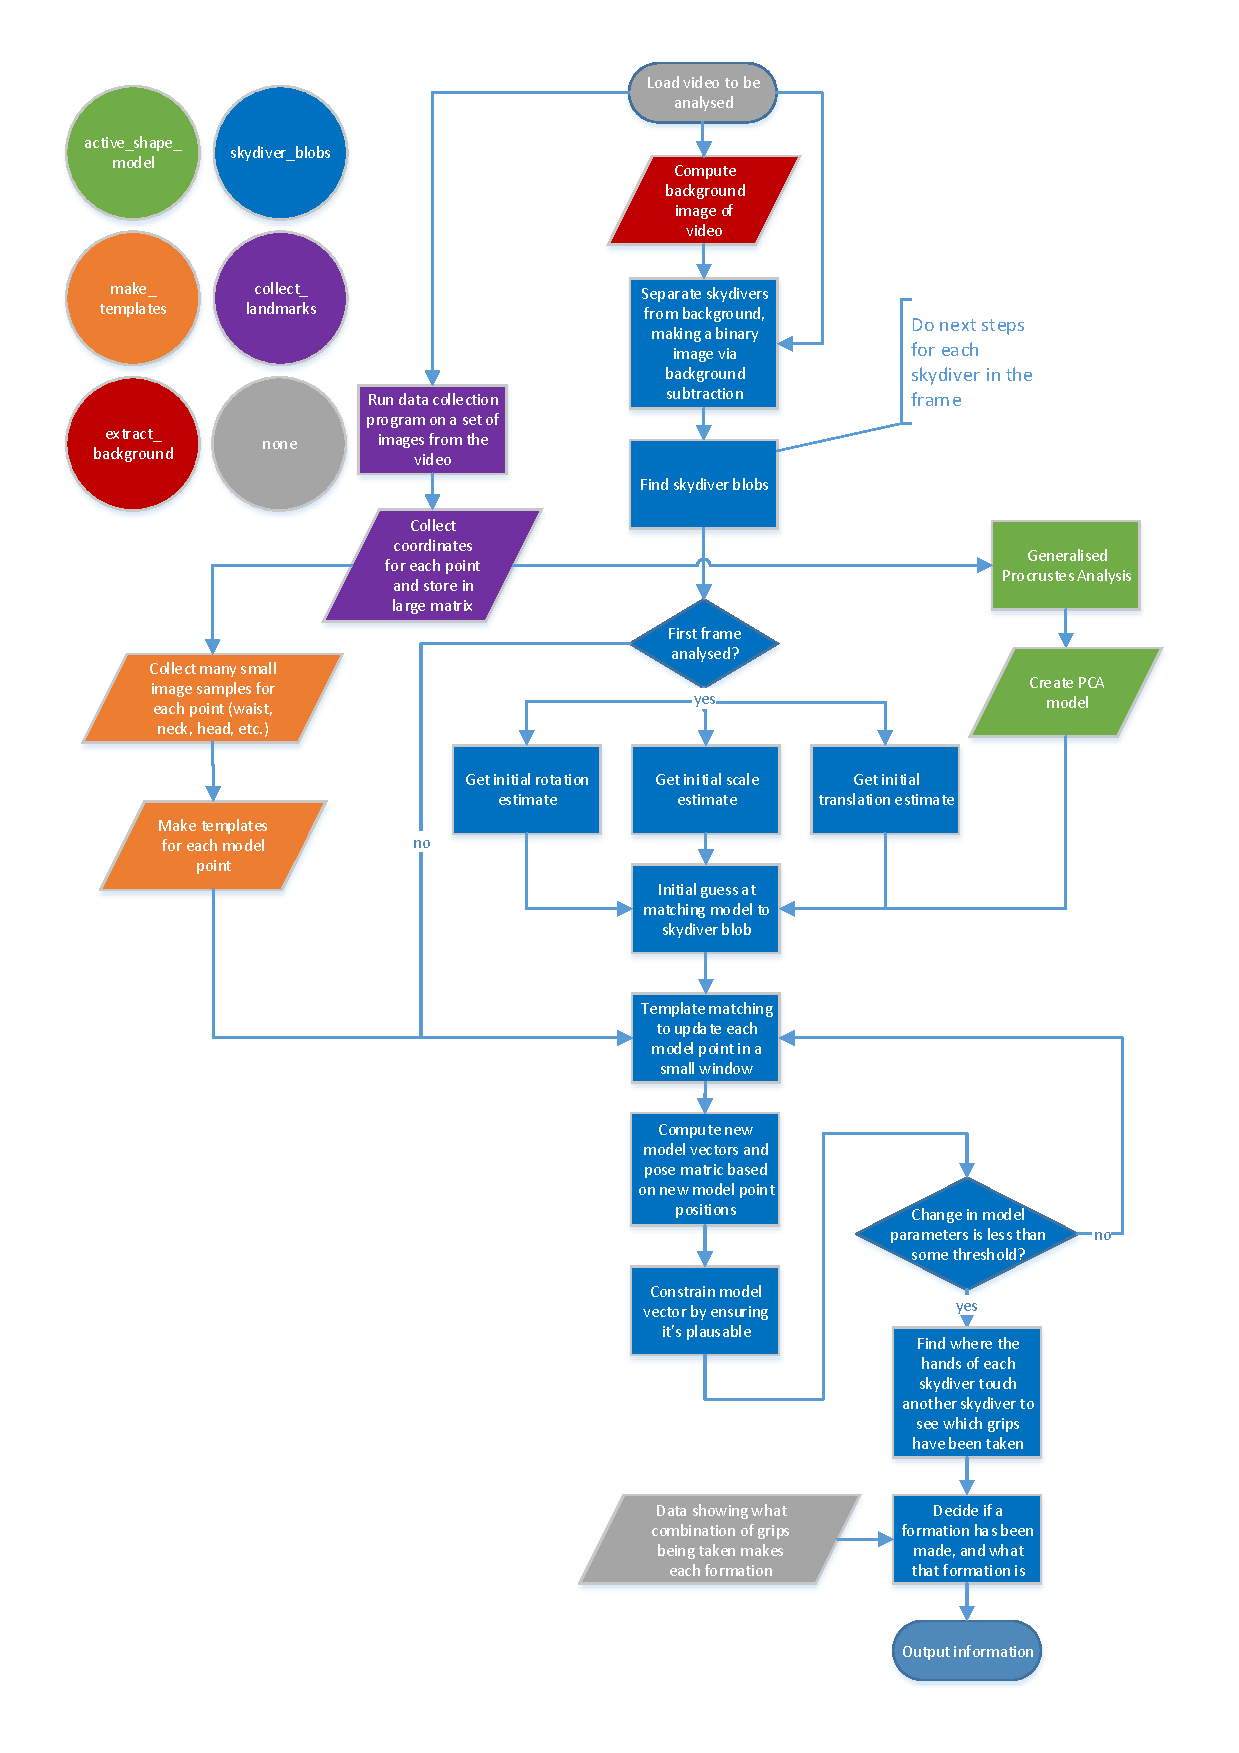
\includepdf[pages={1}]{system_flowchart.pdf}

\chapter{\textbf{B - Initial Gantt Chart}}
\label{appendix:initial_gantt}
%
\begin{figure}[H]
	\centering
	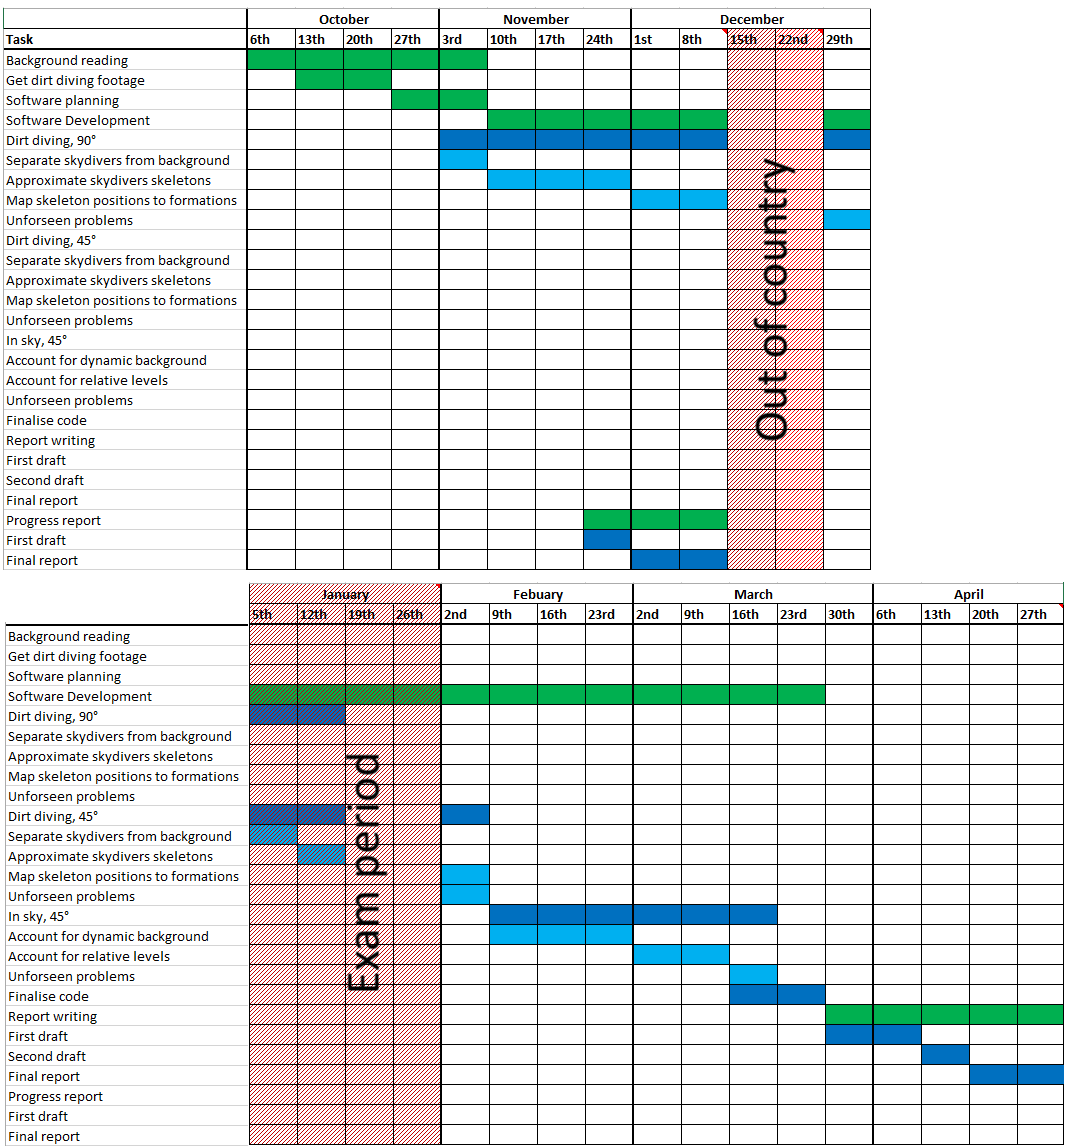
\includegraphics[width=\linewidth]{Gantt_initial_split.png}
	\caption{Initial Gantt Chart}
	\label{fig:gantt_initial}
\end{figure}
%
\chapter{\textbf{C - Revised Gantt Chart}}
\label{appendix:revised_gantt}
%
\begin{figure}[H]
	\centering
	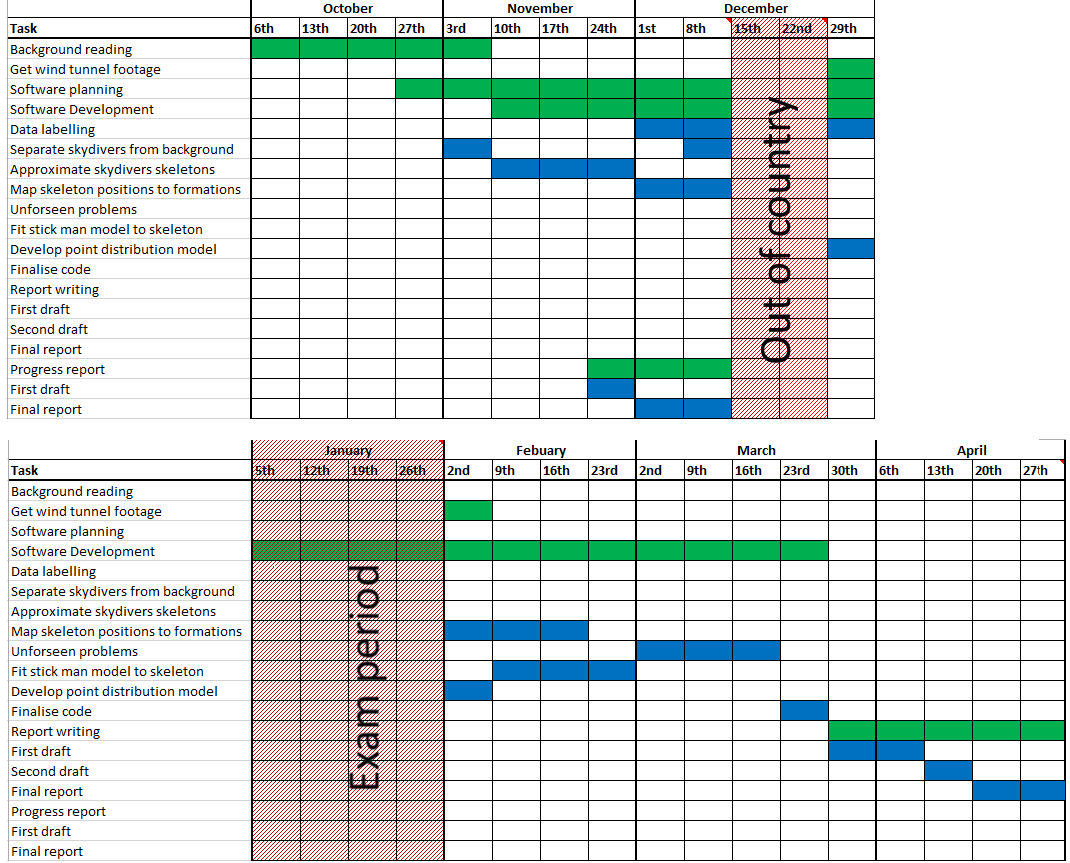
\includegraphics[width=\linewidth]{Gantt_new_split.png}
	\caption{Revised Gantt Chart}
	\label{fig:gantt_new}
\end{figure}
%
%
\chapter{\textbf{D - Progress Report}}
\label{appendix:progress_report}
\includepdf[pages={-}]{progress_report.pdf}
\end{appendices}
%
\end{document}